\title{Operating Systems–2: CS3523 2019\\
Programming Assignment 4: \\
Implement solutions to Readers-Writers and Fair
Readers-Writers problems using Semaphores\\
Report}
\author{Sai Harsha Kottapalli\\CS17BTECH11036}
\date{March 18, 2019}

\documentclass[12pt]{article}
\usepackage{graphicx}
\usepackage[most]{tcolorbox}

\definecolor{bg}{RGB}{220,220,220}

\begin{document}
\maketitle

\section{Aim}
We have to solve the Readers-Writers problem and Fair Readers-Writers problem using Semaphores.\\
We then compare the average and worst-case time taken for each thread to access the critical section (shared
resources).

\section{Design of the Program :}
We use Semaphores to implement the RW and Fair RW problems.
\subsection{Critical Section :}
This part of the code should be accessed by only one writer or multiple readers respectively at a time.
We can avoid race conditions by making sure that no two writer/reader enter their Critical Sections at the same time.
\subsection{Entry Section :}
This part of the code is accessible for all the writers/readers. The job of this code is to make sure only one writer/reader is given access to the critical section at a particular time.
\subsection{Exit Section :}
This part of the code is where the writer/reader has successfully executed the critical section of the program, and will reset the lock so that other writer/readers can now enter the critical section(if any) while this writer/reader completes the remainder section parallelly.
\subsection{Average Waiting Time :}
This is defined as the amount of time each access to critical section takes after requesting for the same.
\subsection{Worst Waiting Time :}
This is defined as the highest amount of time taken by a writer/reader respectively to critical section takes after requesting for the same.

\section{Explanation of program - Common Part}

\subsection{Header files used}
\begin{itemize}
\item \textbf{iostream}\\
Header that defines the standard input/output stream objects
\item \textbf{thread}\\
Used for implementing threads.\\
It defines the class to represent individual threads of execution.\\
A thread of execution is a sequence of instructions that can be executed concurrently with other such sequences in multithreading environments, while sharing a same address space.\\
\item \textbf{fstream}\\
Input/output stream class to operate on files.
\item \textbf{random}\\
This header introduces random number generation facilities.\\
\item \textbf{cstdio}\\
Used for \textbf{sprintf}, that is, for the format in which the time has to be printed to the log file.
\item \textbf{unistd.h}\\
Used for miscellaneous symbolic constants and types, and declares miscellaneous functions - \\
\textbf{localtime} - which is used to get a structure of time, with hours, minutes and seconds.\\
\textbf{time} - For capturing current time which is processed by above command.\\
\textbf{usleep} - accepts microseconds as a parameter to sleep, used for simulating the critical/remainder section.
\item \textbf{string}\\
For processing strings.
\item \textbf{sys/time.h}\\
For using \textbf{gettimeofday()} to obtain the time a producer/consumer has to wait to get access through the lock or semaphore.
\item \textbf{cmath}\\
For using \textbf{floor()} to compare worst case waiting time.
\end{itemize}

\subsection{getInput()}
This is a helper function which helps in keeping the code modular.\\
It reads the value of the following from the input file, specified in ReadMe.txt \\
\begin{itemize}
\item \textbf{Number of writers} - nw
\item \textbf{Number of readers} - nr\\
\item \textbf{Number of times each writer should write} - kw\\
\item \textbf{Number of times each reader should read} - kr\\
\item \textbf{lam1 and lam2}\\
Represents the mean of value of two exponential distribution curves which is to be constructed.\\
Given in milli-seconds.
\end{itemize}

\subsection{writer()}
The writer() function simulates a writer trying to write data to an object.\\
Only one writer at a time, can be inside the CS to avoid synchronization issues.
\subsection{reader()}
The reader() function simulates a reader trying to read data to an object.\\
Only readers at a time, can be inside the CS to avoid synchronization issues.

\subsection{currTime()}
Takes input time$\textunderscore$t structure to generate the time in HH:MM:SS syntax and return this as a string.

\subsection{Other important variables used}
\begin{itemize}
\item \textbf{exponential$\textunderscore$distribution}\\
Produces random non-negative floating-point values x, distributed according to probability density function defined for exponential distribution about the constant rate given as a parameter.
\item \textbf{default$\textunderscore$random$\textunderscore$engine}\\
This is a random number engine class that generates pseudo-random numbers.
\item \textbf{thread *th for writers and readers}\\
th$\textunderscore$w and th$\textunderscore$r are the pointers for storing the array of nw and nr threads respectively. This will be useful for later calling \textbf{join()} to properly exit the threads spawned previously.
\item \textbf{Average and worst waiting times for writers and readers}
Used to calculate the average time as well as worst waiting time, a writer/reader has to wait for getting access to the CS.\\
\end{itemize}

\section{Semaphores}
A semaphore is a variable or abstract data type used to control access to a common resource by multiple processes in a concurrent system such as a multitasking operating system. A semaphore is simply a variable. This variable is used to solve critical section problems and to achieve process synchronization in the multi processing environment.\\
Header file used - \textbf{semaphore.h}\\
The following functions of semaphore in c is  utilized to solve the current problem - 
\begin{itemize}
\item \textbf{sem$\textunderscore$init(sem$\textunderscore$t *sem, int pshared, unsigned int value);}\\
Initializes the unnamed semaphore at the address pointed
to by sem.  The value argument specifies the initial value for the
semaphore.\\
The pshared argument indicates whether this semaphore is to be shared
between the threads of a process, or between processes.
\item \textbf{sem$\textunderscore$wait(sem$\textunderscore$ t *sem);}\\
decrements (locks) the semaphore pointed to by sem.  If
the semaphore's value is greater than zero, then the decrement
proceeds, and the function returns, immediately.  If the semaphore
currently has the value zero, then the call blocks until either it
becomes possible to perform the decrement (i.e., the semaphore value
rises above zero), or a signal handler interrupts the call.
\item \textbf{sem$\textunderscore$post(sem$\textunderscore$t *sem);}\\
increments (unlocks) the semaphore pointed to by sem.  If
the semaphore's value consequently becomes greater than zero, then
another process or thread blocked in a sem$\textunderscore$wait() call will be woken
up and proceed to lock the semaphore.
\item \textbf{sem$\textunderscore$destroy(sem$\textunderscore$t *sem);}\\
destroys the unnamed semaphore at the address pointed to by sem.
\end{itemize}

\section{RW}
\begin{itemize}
\item read$\textunderscore$count is a shared variable which stores number of reader thread currently accessing the CS.
\item I have used two semaphores, namely - rw$\textunderscore$m and mutex.
\item \textbf{rw$\textunderscore$m}\\
This semaphore is initialized to 1.\\
It is used to ensure that only one writer can access CS at any time.\\
\item \textbf{mutex}\\
This semaphore is initialized to 1.\\
It is used to keep count of number of reader threads currently in CS and to correspondingly allow a writer thread to access CS if there are no reader threads currently accessing the CS.\\
\item \textbf{Algorithm :}\\\\

\textbf{Writer}\\
\begin{tcolorbox}[enhanced jigsaw,colback=bg,boxrule=0pt,arc=0pt]
sem$\textunderscore$wait(\&rw$\textunderscore$m);\\
$\char`\\\char`\\$ CS\\
sem$\textunderscore$post(\&rw$\textunderscore$m);\\
$\char`\\\char`\\$ Rem-S
\end{tcolorbox}

\textbf{Reader}\\
\begin{tcolorbox}[enhanced jigsaw,colback=bg,boxrule=0pt,arc=0pt]
sem$\textunderscore$wait(\&mutex);\\
read$\textunderscore$count++;\\
if(read$\textunderscore$count == 1) \{\\
$\hspace*{10mm}$ sem$\textunderscore$wait(\&rw$\textunderscore$m);\\
\}\\
sem$\textunderscore$post(\&mutex);\\
$\char`\\\char`\\$ CS\\
sem$\textunderscore$wait(\&mutex);\\
read$\textunderscore$count--;\\
if(read$\textunderscore$count == 0) \{\\
$\hspace*{10mm}$ sem$\textunderscore$post(\&rw$\textunderscore$m);\\
\}\\
sem$\textunderscore$post(\&mutex);\\
$\char`\\\char`\\$ Rem-S
\end{tcolorbox}
\end{itemize}

\section{Fair RW}
\begin{itemize}
\item I have used three semaphores, namely - in, out, wrt and three variables - ctrin, ctrout, wait.
\item \textbf{in}\\
This semaphore is initialized to 1.\\
\item \textbf{out}\\
This semaphore is initialized to 1.\\
\item \textbf{wrt}\\
This semaphore is initialized to 0.\\
\item \textbf{ctrin}\\
It is an integer initialized to 0.\\
Signifies the number of reader threads which got access to the CS.\\
\item \textbf{ctrout}\\
It is an integer initialized to 0.\\
Signifies the number of reader threads which completed reading the CS.\\
\item \textbf{wait}\\
It is a boolean value initialized to false.\\
Used to check if any writer thread is waiting for access to CS incase any readers are currently inside CS.
\item \textbf{Algorithm :}\\\\

\textbf{Writer}\\
\begin{tcolorbox}[enhanced jigsaw,colback=bg,boxrule=0pt,arc=0pt]
sem$\textunderscore$wait(\&in);\\
sem$\textunderscore$wait(\&out);\\
if(ctrin == ctrout) \{\\
$\hspace*{10mm}$ sem$\textunderscore$post(\&out);\\
\} else \{\\
$\hspace*{10mm}$ wait = 1;\\
$\hspace*{10mm}$ sem$\textunderscore$post(\&out);\\
$\hspace*{10mm}$ sem$\textunderscore$wait(\&wrt);\\
$\hspace*{10mm}$ wait = 0;\\
\}\\
$\char`\\\char`\\$ CS\\
sem$\textunderscore$post(\&in);\\
$\char`\\\char`\\$ Rem-S
\end{tcolorbox}

\textbf{Reader}\\
\begin{tcolorbox}[enhanced jigsaw,colback=bg,boxrule=0pt,arc=0pt]
sem$\textunderscore$wait(\&in);\\
ctrin++;\\
sem$\textunderscore$post(\&in);\\
$\char`\\\char`\\$ CS\\
sem$\textunderscore$wait(\&out);\\
ctrout++;\\
if(wait == 1 \&\& ctrin == ctrout) \{\\
$\hspace*{10mm}$ sem$\textunderscore$post(\&wrt);\\
\}\\
sem$\textunderscore$post(\&out);\\
$\char`\\\char`\\$ Rem-S
\end{tcolorbox}
\end{itemize}


\section{Output}
\begin{itemize}
\item Log files for RW and Fair RW.\\
These store the events which occur throughout the simulation.\\
\\Example : \\
\textit{1st CS Request by Writer Thread 20 at 02:25:57\\}
\textit{1st CS Exit by Writer Thread 1 at 02:25:57\\}
\textit{1st CS Entry by Writer Thread 2 at 02:25:57\\}
\item Average$\textunderscore$time.txt\\
This file stores the average times as well as worst waiting time for writers and readers.\\
The values are in milli-seconds.\\
\\Example: \\
\textit{Average waiting time for writers(ms): 11989.221430}\\
\textit{Average waiting time for readers(ms): 12301.840290}\\
\textit{Worst time for writers to enter CS(ms): 18841.611000}\\
\textit{Worst time for readers to enter CS(ms): 18298.801000}\\
\end{itemize}

\newpage

\section{Comparision}
\subsection{Graphs}
\begin{figure}[ht!]
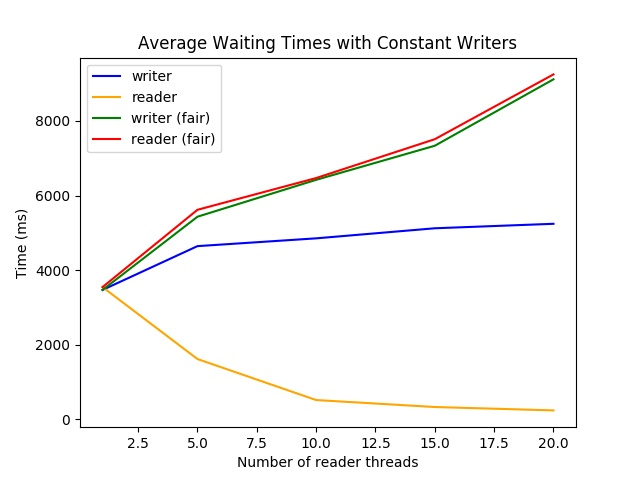
\includegraphics[width=150mm]{1st.jpg}
\caption{Comparision between Average
time taken to enter the CS by reader and writer threads with a constant number of writers for RW and Fair RW}
\end{figure}

\newpage

\begin{figure}[ht!]
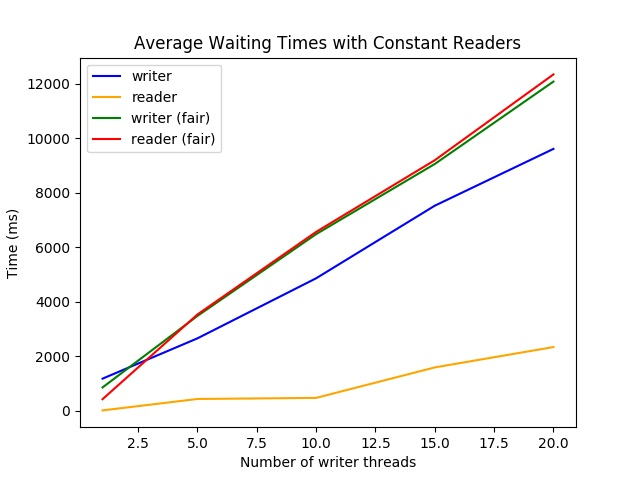
\includegraphics[width=150mm]{2nd.jpg}
\caption{Comparision between Average
time taken to enter the CS by reader and writer threads with a constant number of readers for RW and Fair RW}
\end{figure}

\newpage

\begin{figure}[ht!]
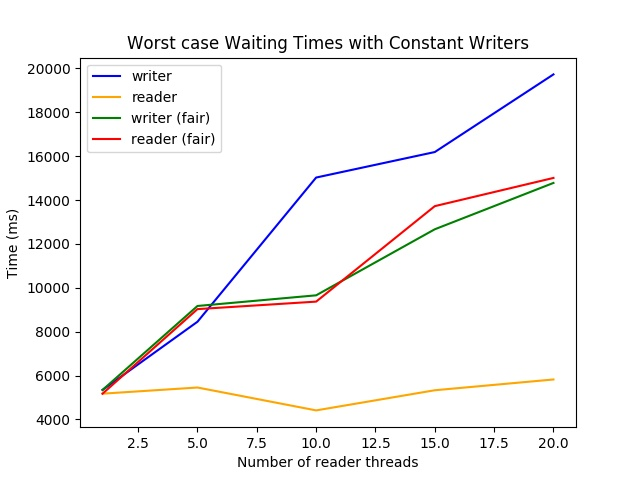
\includegraphics[width=150mm]{3rd.jpg}
\caption{Comparision between worst-case time taken to
enter the CS by reader and writer threads with a constant number of writers for RW and Fair RW}
\end{figure}

\newpage

\begin{figure}[ht!]
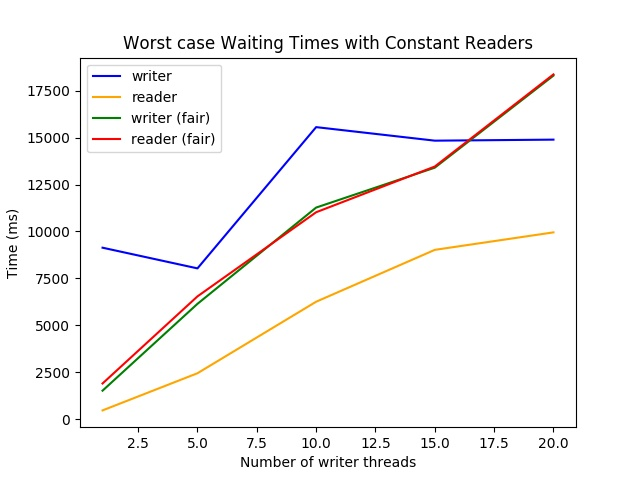
\includegraphics[width=150mm]{4th.jpg}
\caption{Comparision between worst-case time taken to
enter the CS by reader and writer threads with a constant number of readers for RW and Fair RW}
\end{figure}

\newpage

\subsection{Notes}
\begin{enumerate}
\item Parameters used for test cases:\\
nw = 1, 5, 10, 15, 20\\
nr = 1, 5, 10, 15, 20\\
kw = 10\\
kr = 10\\
$\Lambda _1$ = 500 milli-seconds and $\Lambda _2$ = 800 milli-seconds,\\
\item Each of the plotted points is the average of 5 testcases.\\
\item Average waiting times with constant writers
	\begin{itemize}
	\item As we increase the number of reader threads, we notice that all the threads except reader thread show an increase in waiting times.
	\item As for reader, the waiting time decreased with increase of reader threads.
	\item There is almost no difference between the waiting times of the reader and
				writer threads for Fair Readers-Writers when compared to Normal Readers-Writers which
				shows the effectiveness of the Fair RW algorithm.
	\item The starvation of writers in RW algorithm can also be noticed here.
	\item Overhead in Fair RW algo, also accounts for increased waiting times, in their case.
	\end{itemize}
\item Average waiting times with constant readers
	\begin{itemize}
	\item This also follows similar trend as previous graph except even readers waiting time increases with 				increase in writer threads.
	\item The common starting point is lower than previous graph, this is because the number of writer threads are lower than before.\\
	The writer threads are responsible for other waiting times as well, because this follows a convoy effect.
	\item The starvation of writers in RW algorithm can also be noticed here.
	\end{itemize}
	\item Worst case waiting times with constant writers/readers.
	\begin{itemize}
	\item With increase in number of threads, the worst case waiting times also increases.
	\item The worst case waiting time for Fair RW is very close for writers and readers, which shows that starvation is taken care of.\\
	As for normal RW, the writer are starving so they have much higher waiting time when compared to readers.
	\item The difference in starting points in the two graphs is due to the same reason as stated earlier - because of writer threads and their convoy effect.
	\end{itemize}
\end{enumerate}

\end{document}